%-*-latex-*-
\sectionthree{Probabilistic or random experiments}
\begin{python0}
from solutions import *; clear()
\end{python0}

\subsection{What is probability?}

First let me talk about probability informally.

If you roll a fair die, there's a one-in-six chance that you'll get a 5.
What does that mean?

It does not mean that if you roll that die 6 times,
you'll see 5 exactly once.
The \lq\lq one-in-six chance" means that if you roll
the die $n$ times, then
\[
\frac{\text{number of rolls that give 5}}{\text{total number of rolls}}
\approx \frac{1}{6}
\]
and furthermore the larger the $n$, the closer you get to $1/6$.
Instead of saying \lq\lq one-in-six chance that", one would also say
\lq\lq there's a probability of 1/6 that ...".

If you are interested in the probability of get a 5 or 6, then
you roll your die as many times as you can and compute
\[
\frac{\text{number of rolls that give 5 or 6}}{\text{total number of rolls}}
\]
and you'll see that the number you want is $1/3$.

A die is fair if the probability of getting any face is the same for all
faces.
Likewise if you are tossing coin, a coin is fair if the probability of
getting a head is the same as the probability of getting a tail.
If I don't say so, then all die, coin, or any \lq\lq random calculating
device" are fair.

The act of rolling a die and gather data from this
\lq\lq random device" is called a random experiment.

Here's another type of questions you'll see when working random experiments:
What is the average value when you roll a die?
The \lq\lq average value" here
means the average of the values you get for a number of rolls.
\[
\frac{\text{sum of rolls}}{\text{total number of rolls}}
\]
Go ahead and get a die and roll it 100 times.
You'll see that your average is 3.5.
Why?
Suppose you roll your die $n$ times.
Let's say
the number of times you get a 1 is $n_1$,
the number of times you get a 2 is $n_2$,
etc.
Then the average value is
\begin{align*}
  \frac{\text{sum of rolls}}{\text{total number of rolls}}
  &= \frac{
    n_1 \cdot 1
    +
    n_2 \cdot 2
    +
    \cdots
    +
    n_6 \cdot 6
  }{n}
  \\
  &= \frac{n_1}{n} \cdot 1
  + \cdots + 
  \frac{n_6}{n} \cdot 6
\end{align*}
But of course $n_i/n = 1/6$ if $n$ is huge since $n_i/n$ is the
probability of getting $i$.
Therefore the average value of a die roll is $3.5$.
Get it?

In the case of rolling a fair die 
the probability of getting $k$ (for $k = 1, 2, 3$, ..., or $6$) is
$1/6$.
So all values have the same probability.
Likewise for a fair coin the probability is the same
for getting a head and getting a tail.
For instance one can make a biased die where 6 occurs more frequently
than the other numbers.


%-*-latex-*-

\begin{ex} 
  \label{ex:prob-00}
  \tinysidebar{\debug{exercises/{disc-prob-28/question.tex}}}

  \solutionlink{sol:prob-00}
  \qed
\end{ex} 
\begin{python0}
from solutions import *
add(label="ex:prob-00",
    srcfilename='exercises/discrete-probability/prob-00/answer.tex') 
\end{python0}

%-*-latex-*-

\begin{ex} 
  \label{ex:prob-00}
  \tinysidebar{\debug{exercises/{disc-prob-28/question.tex}}}

  \solutionlink{sol:prob-00}
  \qed
\end{ex} 
\begin{python0}
from solutions import *
add(label="ex:prob-00",
    srcfilename='exercises/discrete-probability/prob-00/answer.tex') 
\end{python0}





\subsection{Coin toss experiments}

If you have a coin, you can toss it and get either head or tail.
(It won't land on its side ... unless if you have
an extremely \textit{ thick} coin ...)
If the coin is fair, half the time you will get a head and 
half the time you will get a tail.
Let's call each toss a random experiment and let's
call the result of your toss the outcome of the experiment.
The two possible outcomes are getting a head and getting tail.
I'll create symbols to denote these two outcomes:
\[
  \HEAD \text{ and } \TAIL
\]
If you're the gambling kind, you know that in fact there's a slightly
higher chance that the head falls face down so that 
there's a slightly higher chance of getting the tail.
Let's ignore this fact and just assume that our coin is absolutely fair.

If you don't have a fair coin, you can write a 
program to simulate the tossing of the coin like this one
in your favorite programming language (C/\cpp, Java, Python, what-have-you):
{\footnotesize
\includesourcenonumbers{tossfaircoin1.py}
}
Here's my output when I run the program:
%-*-latex-*-
{\footnotesize \begin{Verbatim}[frame=single,fontsize=\small]
[student@localhost discrete-probability] python tossfaircoin1.py
experiment 0 ... outcome: HEAD
experiment 1 ... outcome: TAIL
experiment 2 ... outcome: HEAD
experiment 3 ... outcome: TAIL
experiment 4 ... outcome: HEAD
experiment 5 ... outcome: TAIL
experiment 6 ... outcome: TAIL
experiment 7 ... outcome: TAIL
experiment 8 ... outcome: TAIL
experiment 9 ... outcome: TAIL
experiment 10 ... outcome: TAIL
experiment 11 ... outcome: HEAD
experiment 12 ... outcome: HEAD
experiment 13 ... outcome: TAIL
experiment 14 ... outcome: HEAD
experiment 15 ... outcome: HEAD
experiment 16 ... outcome: HEAD
experiment 17 ... outcome: TAIL
experiment 18 ... outcome: TAIL
experiment 19 ... outcome: HEAD
\end{Verbatim}
}


Much better isn't it?
Not because I don't have a quarter, but because I can easily
do a million coin-toss experiments in a split second by changing \verb!n!.
I can also collect all the outcomes and tabulate:
{\small
\includesourcenonumbers{tossfaircoin2.py}
}
Here's my output when I run the program:
\begin{center}
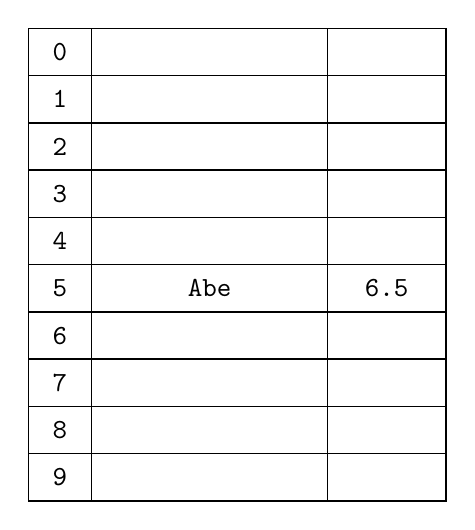
\begin{tikzpicture}

\draw (1.4, 0.7)
  node[draw, line width=0.02cm, , color=black,
       rounded corners=0cm, inner sep=0cm] {

\begin{minipage}[t][0.6cm]{0.8cm}
\mbox{}

\end{minipage}

};\draw (1.4, 0.7) node[color=black] {{\texttt{0}}};
\draw (3.3, 0.7)
  node[draw, line width=0.02cm, , color=black,
       rounded corners=0cm, inner sep=0cm] {

\begin{minipage}[t][0.6cm]{3.0cm}
\mbox{}

\end{minipage}

};\draw (3.3, 0.7) node[color=black] {{\texttt{}}};
\draw (5.55, 0.7)
  node[draw, line width=0.02cm, , color=black,
       rounded corners=0cm, inner sep=0cm] {

\begin{minipage}[t][0.6cm]{1.5cm}
\mbox{}

\end{minipage}

};\draw (5.55, 0.7) node[color=black] {{\texttt{}}};
\draw (1.4, 0.09999999999999987)
  node[draw, line width=0.02cm, , color=black,
       rounded corners=0cm, inner sep=0cm] {

\begin{minipage}[t][0.6cm]{0.8cm}
\mbox{}

\end{minipage}

};\draw (1.4, 0.09999999999999987) node[color=black] {{\texttt{1}}};
\draw (3.3, 0.09999999999999987)
  node[draw, line width=0.02cm, , color=black,
       rounded corners=0cm, inner sep=0cm] {

\begin{minipage}[t][0.6cm]{3.0cm}
\mbox{}

\end{minipage}

};\draw (3.3, 0.09999999999999987) node[color=black] {{\texttt{}}};
\draw (5.55, 0.09999999999999987)
  node[draw, line width=0.02cm, , color=black,
       rounded corners=0cm, inner sep=0cm] {

\begin{minipage}[t][0.6cm]{1.5cm}
\mbox{}

\end{minipage}

};\draw (5.55, 0.09999999999999987) node[color=black] {{\texttt{}}};
\draw (1.4, -0.5000000000000002)
  node[draw, line width=0.02cm, , color=black,
       rounded corners=0cm, inner sep=0cm] {

\begin{minipage}[t][0.6cm]{0.8cm}
\mbox{}

\end{minipage}

};\draw (1.4, -0.5000000000000002) node[color=black] {{\texttt{2}}};
\draw (3.3, -0.5000000000000002)
  node[draw, line width=0.02cm, , color=black,
       rounded corners=0cm, inner sep=0cm] {

\begin{minipage}[t][0.6cm]{3.0cm}
\mbox{}

\end{minipage}

};\draw (3.3, -0.5000000000000002) node[color=black] {{\texttt{}}};
\draw (5.55, -0.5000000000000002)
  node[draw, line width=0.02cm, , color=black,
       rounded corners=0cm, inner sep=0cm] {

\begin{minipage}[t][0.6cm]{1.5cm}
\mbox{}

\end{minipage}

};\draw (5.55, -0.5000000000000002) node[color=black] {{\texttt{}}};
\draw (1.4, -1.1000000000000003)
  node[draw, line width=0.02cm, , color=black,
       rounded corners=0cm, inner sep=0cm] {

\begin{minipage}[t][0.6cm]{0.8cm}
\mbox{}

\end{minipage}

};\draw (1.4, -1.1000000000000003) node[color=black] {{\texttt{3}}};
\draw (3.3, -1.1000000000000003)
  node[draw, line width=0.02cm, , color=black,
       rounded corners=0cm, inner sep=0cm] {

\begin{minipage}[t][0.6cm]{3.0cm}
\mbox{}

\end{minipage}

};\draw (3.3, -1.1000000000000003) node[color=black] {{\texttt{}}};
\draw (5.55, -1.1000000000000003)
  node[draw, line width=0.02cm, , color=black,
       rounded corners=0cm, inner sep=0cm] {

\begin{minipage}[t][0.6cm]{1.5cm}
\mbox{}

\end{minipage}

};\draw (5.55, -1.1000000000000003) node[color=black] {{\texttt{}}};
\draw (1.4, -1.7000000000000002)
  node[draw, line width=0.02cm, , color=black,
       rounded corners=0cm, inner sep=0cm] {

\begin{minipage}[t][0.6cm]{0.8cm}
\mbox{}

\end{minipage}

};\draw (1.4, -1.7000000000000002) node[color=black] {{\texttt{4}}};
\draw (3.3, -1.7000000000000002)
  node[draw, line width=0.02cm, , color=black,
       rounded corners=0cm, inner sep=0cm] {

\begin{minipage}[t][0.6cm]{3.0cm}
\mbox{}

\end{minipage}

};\draw (3.3, -1.7000000000000002) node[color=black] {{\texttt{}}};
\draw (5.55, -1.7000000000000002)
  node[draw, line width=0.02cm, , color=black,
       rounded corners=0cm, inner sep=0cm] {

\begin{minipage}[t][0.6cm]{1.5cm}
\mbox{}

\end{minipage}

};\draw (5.55, -1.7000000000000002) node[color=black] {{\texttt{}}};
\draw (1.4, -2.3000000000000003)
  node[draw, line width=0.02cm, , color=black,
       rounded corners=0cm, inner sep=0cm] {

\begin{minipage}[t][0.6cm]{0.8cm}
\mbox{}

\end{minipage}

};\draw (1.4, -2.3000000000000003) node[color=black] {{\texttt{5}}};
\draw (3.3, -2.3000000000000003)
  node[draw, line width=0.02cm, , color=black,
       rounded corners=0cm, inner sep=0cm] {

\begin{minipage}[t][0.6cm]{3.0cm}
\mbox{}

\end{minipage}

};\draw (3.3, -2.3000000000000003) node[color=black] {{\texttt{Abe}}};
\draw (5.55, -2.3000000000000003)
  node[draw, line width=0.02cm, , color=black,
       rounded corners=0cm, inner sep=0cm] {

\begin{minipage}[t][0.6cm]{1.5cm}
\mbox{}

\end{minipage}

};\draw (5.55, -2.3000000000000003) node[color=black] {{\texttt{6.5}}};
\draw (1.4, -2.9000000000000004)
  node[draw, line width=0.02cm, , color=black,
       rounded corners=0cm, inner sep=0cm] {

\begin{minipage}[t][0.6cm]{0.8cm}
\mbox{}

\end{minipage}

};\draw (1.4, -2.9000000000000004) node[color=black] {{\texttt{6}}};
\draw (3.3, -2.9000000000000004)
  node[draw, line width=0.02cm, , color=black,
       rounded corners=0cm, inner sep=0cm] {

\begin{minipage}[t][0.6cm]{3.0cm}
\mbox{}

\end{minipage}

};\draw (3.3, -2.9000000000000004) node[color=black] {{\texttt{}}};
\draw (5.55, -2.9000000000000004)
  node[draw, line width=0.02cm, , color=black,
       rounded corners=0cm, inner sep=0cm] {

\begin{minipage}[t][0.6cm]{1.5cm}
\mbox{}

\end{minipage}

};\draw (5.55, -2.9000000000000004) node[color=black] {{\texttt{}}};
\draw (1.4, -3.500000000000001)
  node[draw, line width=0.02cm, , color=black,
       rounded corners=0cm, inner sep=0cm] {

\begin{minipage}[t][0.6cm]{0.8cm}
\mbox{}

\end{minipage}

};\draw (1.4, -3.500000000000001) node[color=black] {{\texttt{7}}};
\draw (3.3, -3.500000000000001)
  node[draw, line width=0.02cm, , color=black,
       rounded corners=0cm, inner sep=0cm] {

\begin{minipage}[t][0.6cm]{3.0cm}
\mbox{}

\end{minipage}

};\draw (3.3, -3.500000000000001) node[color=black] {{\texttt{}}};
\draw (5.55, -3.500000000000001)
  node[draw, line width=0.02cm, , color=black,
       rounded corners=0cm, inner sep=0cm] {

\begin{minipage}[t][0.6cm]{1.5cm}
\mbox{}

\end{minipage}

};\draw (5.55, -3.500000000000001) node[color=black] {{\texttt{}}};
\draw (1.4, -4.1000000000000005)
  node[draw, line width=0.02cm, , color=black,
       rounded corners=0cm, inner sep=0cm] {

\begin{minipage}[t][0.6cm]{0.8cm}
\mbox{}

\end{minipage}

};\draw (1.4, -4.1000000000000005) node[color=black] {{\texttt{8}}};
\draw (3.3, -4.1000000000000005)
  node[draw, line width=0.02cm, , color=black,
       rounded corners=0cm, inner sep=0cm] {

\begin{minipage}[t][0.6cm]{3.0cm}
\mbox{}

\end{minipage}

};\draw (3.3, -4.1000000000000005) node[color=black] {{\texttt{}}};
\draw (5.55, -4.1000000000000005)
  node[draw, line width=0.02cm, , color=black,
       rounded corners=0cm, inner sep=0cm] {

\begin{minipage}[t][0.6cm]{1.5cm}
\mbox{}

\end{minipage}

};\draw (5.55, -4.1000000000000005) node[color=black] {{\texttt{}}};
\draw (1.4, -4.7)
  node[draw, line width=0.02cm, , color=black,
       rounded corners=0cm, inner sep=0cm] {

\begin{minipage}[t][0.6cm]{0.8cm}
\mbox{}

\end{minipage}

};\draw (1.4, -4.7) node[color=black] {{\texttt{9}}};
\draw (3.3, -4.7)
  node[draw, line width=0.02cm, , color=black,
       rounded corners=0cm, inner sep=0cm] {

\begin{minipage}[t][0.6cm]{3.0cm}
\mbox{}

\end{minipage}

};\draw (3.3, -4.7) node[color=black] {{\texttt{}}};
\draw (5.55, -4.7)
  node[draw, line width=0.02cm, , color=black,
       rounded corners=0cm, inner sep=0cm] {

\begin{minipage}[t][0.6cm]{1.5cm}
\mbox{}

\end{minipage}

};\draw (5.55, -4.7) node[color=black] {{\texttt{}}};
\end{tikzpicture}

\end{center}



%-*-latex-*-

\begin{ex} 
  \label{ex:prob-00}
  \tinysidebar{\debug{exercises/{disc-prob-28/question.tex}}}

  \solutionlink{sol:prob-00}
  \qed
\end{ex} 
\begin{python0}
from solutions import *
add(label="ex:prob-00",
    srcfilename='exercises/discrete-probability/prob-00/answer.tex') 
\end{python0}


Of course if your \verb!N! is really, really, really huge,
you will find that the probability of getting a head is 0.5 and 
the probability of getting a tail is 0.5.

Here's a function (derived by simulation) 
that gives us the probability for each possible outcome
of our experiment:
\includesourcenonumbers{tossfaircoin3.py}
I've increase \verb!n! to 1000 and 
also commented out the printing of each experiment.
Here's my output when I run the program:
\begin{center}
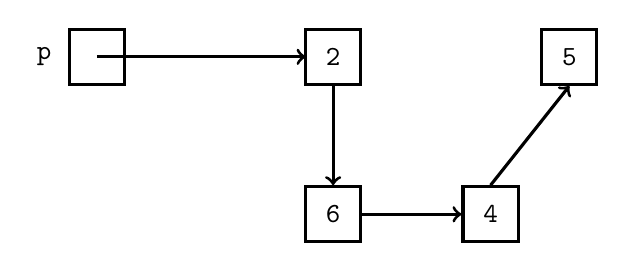
\begin{tikzpicture}

\draw (0.35, 0.35)
  node[draw, line width=0.04cm, , color=black,
       rounded corners=0cm, inner sep=0cm] {

\begin{minipage}[t][0.7cm]{0.7cm}
\mbox{}

\end{minipage}

};\draw (0.35, 0.35) node[color=black] {{\texttt{2}}};
\draw (0.35, -1.65)
  node[draw, line width=0.04cm, , color=black,
       rounded corners=0cm, inner sep=0cm] {

\begin{minipage}[t][0.7cm]{0.7cm}
\mbox{}

\end{minipage}

};\draw (0.35, -1.65) node[color=black] {{\texttt{6}}};
\draw (2.35, -1.65)
  node[draw, line width=0.04cm, , color=black,
       rounded corners=0cm, inner sep=0cm] {

\begin{minipage}[t][0.7cm]{0.7cm}
\mbox{}

\end{minipage}

};\draw (2.35, -1.65) node[color=black] {{\texttt{4}}};
\draw (3.35, 0.35)
  node[draw, line width=0.04cm, , color=black,
       rounded corners=0cm, inner sep=0cm] {

\begin{minipage}[t][0.7cm]{0.7cm}
\mbox{}

\end{minipage}

};\draw (3.35, 0.35) node[color=black] {{\texttt{5}}};\draw[line width=0.04cm,black,->] (0.35,-0.02) to  (0.35,-1.28);
\draw[line width=0.04cm,black,->] (0.72,-1.65) to  (1.98,-1.65);
\draw[line width=0.04cm,black,->] (2.35,-1.28) to  (3.35,-0.02);

\draw (-2.65, 0.35)
  node[draw, line width=0.04cm, , color=black,
       rounded corners=0cm, inner sep=0cm] {

\begin{minipage}[t][0.7cm]{0.7cm}
\mbox{}

\end{minipage}

};\draw (-2.65, 0.35) node[color=black] {{\texttt{}}};\draw[line width=0.04cm,black,->] (-2.65,0.35) to  (0,0.35);

\draw (-3.32, 0.35)
  node[draw, line width=0.04cm, , color=white,
       rounded corners=0cm, inner sep=0cm] {

\begin{minipage}[t][0.1cm]{0.1cm}
\mbox{}

\end{minipage}

};\draw (-3.32, 0.35) node[color=black] {{\texttt{p}}};
\end{tikzpicture}

\end{center}



Of course if we assume from the beginning that our coin is fair we can 
save the trouble of the computation:
\includesourcenonumbers{tossfaircoin4.py}
Here's my output when I run the program:
\begin{center}
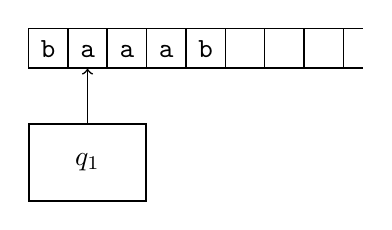
\begin{tikzpicture}

\draw (0.25, 0.25)
  node[draw, line width=0.02cm, , color=black,
       rounded corners=0cm, inner sep=0cm] {

\begin{minipage}[t][0.5cm]{0.5cm}
\mbox{}

\end{minipage}

};\draw (0.25, 0.25) node[color=black] {{\vphantom{baaab\SPACE\SPACE\SPACE}\texttt{b}}};
\draw (0.75, 0.25)
  node[draw, line width=0.02cm, , color=black,
       rounded corners=0cm, inner sep=0cm] {

\begin{minipage}[t][0.5cm]{0.5cm}
\mbox{}

\end{minipage}

};\draw (0.75, 0.25) node[color=black] {{\vphantom{baaab\SPACE\SPACE\SPACE}\texttt{a}}};
\draw (1.25, 0.25)
  node[draw, line width=0.02cm, , color=black,
       rounded corners=0cm, inner sep=0cm] {

\begin{minipage}[t][0.5cm]{0.5cm}
\mbox{}

\end{minipage}

};\draw (1.25, 0.25) node[color=black] {{\vphantom{baaab\SPACE\SPACE\SPACE}\texttt{a}}};
\draw (1.75, 0.25)
  node[draw, line width=0.02cm, , color=black,
       rounded corners=0cm, inner sep=0cm] {

\begin{minipage}[t][0.5cm]{0.5cm}
\mbox{}

\end{minipage}

};\draw (1.75, 0.25) node[color=black] {{\vphantom{baaab\SPACE\SPACE\SPACE}\texttt{a}}};
\draw (2.25, 0.25)
  node[draw, line width=0.02cm, , color=black,
       rounded corners=0cm, inner sep=0cm] {

\begin{minipage}[t][0.5cm]{0.5cm}
\mbox{}

\end{minipage}

};\draw (2.25, 0.25) node[color=black] {{\vphantom{baaab\SPACE\SPACE\SPACE}\texttt{b}}};
\draw (2.75, 0.25)
  node[draw, line width=0.02cm, , color=black,
       rounded corners=0cm, inner sep=0cm] {

\begin{minipage}[t][0.5cm]{0.5cm}
\mbox{}

\end{minipage}

};\draw (2.75, 0.25) node[color=black] {{\vphantom{baaab\SPACE\SPACE\SPACE}\texttt{\SPACE}}};
\draw (3.25, 0.25)
  node[draw, line width=0.02cm, , color=black,
       rounded corners=0cm, inner sep=0cm] {

\begin{minipage}[t][0.5cm]{0.5cm}
\mbox{}

\end{minipage}

};\draw (3.25, 0.25) node[color=black] {{\vphantom{baaab\SPACE\SPACE\SPACE}\texttt{\SPACE}}};
\draw (3.75, 0.25)
  node[draw, line width=0.02cm, , color=black,
       rounded corners=0cm, inner sep=0cm] {

\begin{minipage}[t][0.5cm]{0.5cm}
\mbox{}

\end{minipage}

};\draw (3.75, 0.25) node[color=black] {{\vphantom{baaab\SPACE\SPACE\SPACE}\texttt{\SPACE}}};\draw[line width=0.02cm,black] (4.0,0.5) to  (4.25,0.5);
\draw[line width=0.02cm,black] (4.0,0.0) to  (4.25,0.0);

\draw (0.75, -1.2)
  node[draw, line width=0.02cm, , color=black,
       rounded corners=0cm, inner sep=0cm] {

\begin{minipage}[t][0.98cm]{1.48cm}
\mbox{}

\end{minipage}

};\draw (0.75, -1.2) node[color=black] {$q_1$};\draw[line width=0.02cm,black,->] (0.75,-0.7) to  (0.75,-0.47) to  (0.75,-0.47) to  (0.75,-0.01);
\end{tikzpicture}

\end{center}



Of course when \verb!n! gets larger and larger, the probability function
derived using simulations will match this new \lq\lq theoretically'' derived
function.

%-*-latex-*-

\begin{ex} 
  \label{ex:prob-00}
  \tinysidebar{\debug{exercises/{disc-prob-28/question.tex}}}

  \solutionlink{sol:prob-00}
  \qed
\end{ex} 
\begin{python0}
from solutions import *
add(label="ex:prob-00",
    srcfilename='exercises/discrete-probability/prob-00/answer.tex') 
\end{python0}

%-*-latex-*-

\begin{ex} 
  \label{ex:prob-00}
  \tinysidebar{\debug{exercises/{disc-prob-28/question.tex}}}

  \solutionlink{sol:prob-00}
  \qed
\end{ex} 
\begin{python0}
from solutions import *
add(label="ex:prob-00",
    srcfilename='exercises/discrete-probability/prob-00/answer.tex') 
\end{python0}

%-*-latex-*-

\begin{ex} 
  \label{ex:prob-00}
  \tinysidebar{\debug{exercises/{disc-prob-28/question.tex}}}

  \solutionlink{sol:prob-00}
  \qed
\end{ex} 
\begin{python0}
from solutions import *
add(label="ex:prob-00",
    srcfilename='exercises/discrete-probability/prob-00/answer.tex') 
\end{python0}


I abstract the coin toss experiment as follows:
Let $S = \{\HEAD, \TAIL\}$ represent all possible outcomes of
my coin toss experiment.
$S$ is the called the \defone{sample space} of my random experiment.
$\HEAD$ and $\TAIL$ are called
the \defone{outcomes} of my experiment.
I define a function
\[
  p : S \rightarrow \R 
\]
such that $p(\HEAD)$ gives us the chance that
a coin toss will give us a head and
$p(\TAIL)$ gives us the chance of getting a tail.
So if the coin is fair, I would have
\[
  p(\HEAD) = 1/2 = p(\TAIL)
\]
$p$ is called a
\defterm{probability distribution function}\index{probability distribution function}\tinysidebar{probability distribution function \\ pdf}
(\defterm{pdf}\index{pdf}):
it distributes $1$ to all outcomes:
\[
1 = p(\HEAD) + p(\TAIL) = \sum_{x \in S} p(x)
\]
$p$ is also called a
\defterm{probability function}\index{probability function}\tinysidebar{probability function \\ probability mass function}
or a 
\defterm{probability mass function}\index{probability mass function}.




\newpage
\subsection{Die rolls}

When you roll a die, you get the face value of the roll, i.e.,
the number of dots on the top surface of the die, you
get one of the following:
\[
\text{
\texttt{ONE},
\texttt{TWO},
\texttt{THREE},
\texttt{FOUR},
\texttt{FIVE},
\texttt{SIX},
}
\]
Assuming that the die is fair and you roll the die a huge
number of times, you will see that approximately 1/6 of the 
rolls will give you a \texttt{ONE}
(and likewise for the other cases.)

I can assign 1/6 to \texttt{ONE} to indicate that the 
proportion of rolls that gives me \texttt{ONE}.
Likewise for the other cases.
This is basically a function
\[
p : \{\texttt{ONE},
\texttt{TWO},
\texttt{THREE},
\texttt{FOUR},
\texttt{FIVE},
\texttt{SIX}
\}
\rightarrow [0,1]
\]
such that 
\begin{align*}
p(\texttt{ONE}) &= 1/6 \\
p(\texttt{TWO}) &= 1/6 \\
p(\texttt{THREE}) &= 1/6 \\
p(\texttt{FOUR}) &= 1/6 \\
p(\texttt{FIVE}) &= 1/6 \\
p(\texttt{SIX}) &= 1/6
\end{align*}
As in the previous subsection, the set 
$S = \{
\texttt{ONE},
\texttt{TWO},
\texttt{THREE},
\texttt{FOUR},
\texttt{FIVE},
\texttt{SIX}
\}$ 
is called the set of outcomes or the sample space
of my experiment of rolling a die.
Note that
\[
\sum_{x \in S} p(x) = 1
\]

For us, our sample space is a finite set (you can also 
talk about probability theory for non-finite sets.) 


%-*-latex-*-

\begin{ex} 
  \label{ex:prob-00}
  \tinysidebar{\debug{exercises/{disc-prob-28/question.tex}}}

  \solutionlink{sol:prob-00}
  \qed
\end{ex} 
\begin{python0}
from solutions import *
add(label="ex:prob-00",
    srcfilename='exercises/discrete-probability/prob-00/answer.tex') 
\end{python0}

%-*-latex-*-

\begin{ex} 
  \label{ex:prob-00}
  \tinysidebar{\debug{exercises/{disc-prob-28/question.tex}}}

  \solutionlink{sol:prob-00}
  \qed
\end{ex} 
\begin{python0}
from solutions import *
add(label="ex:prob-00",
    srcfilename='exercises/discrete-probability/prob-00/answer.tex') 
\end{python0}


A probability distribution function is \defone{uniform}
if $p(x)$ is the same for all $x$ in the sample space of the function.
When I say that I'm rolling a \defone{fair} die, I mean that the probability
function for the experiment (of rolling the die) is uniform.

%-*-latex-*-

\begin{ex} 
  \label{ex:prob-00}
  \tinysidebar{\debug{exercises/{disc-prob-28/question.tex}}}

  \solutionlink{sol:prob-00}
  \qed
\end{ex} 
\begin{python0}
from solutions import *
add(label="ex:prob-00",
    srcfilename='exercises/discrete-probability/prob-00/answer.tex') 
\end{python0}


Instead of asking the probability of getting a \texttt{SIX} when
I roll a die, I might be interested in getting \texttt{ONE} or \texttt{SIX}.
In general, a subset $A$ of the set of all outcomes is called an 
\defone{event}.
In that case, I will write $p(A)$ or $p[A]$ for
\[
p(A) = \sum_{x \in A} p(x)
\]
So for instance in the case of our die,
\[
p[\{\texttt{ONE}, \texttt{SIX}\}]
= p(\texttt{ONE}) + p(\texttt{SIX})
= 1/6 + 1/6 = 1/3
\]

Let $A$ and $B$ be events of an experiment with sample space $S$
and probability distribution function $p$.
Then
\[
p[A \cup B] \leq p[A] + p[B]
\]
This means that if we know a lot about the probability of $A$ and 
probability of $B$, but we're not very sure about the common
events of $A$ and $B$, we can still bound the probability of $A \cup B$.
If we do know something about the probability of $A \cap B$, then we have
\[
p[A \cup B] = p[A] + p[B] - p[A \cap B]
\]

If $A \cap B = \emptyset$, we get
\[
p[A \cup B] = p[A] + p[B]
\]
Clearly we also have
\[
p[\emptyset] = 0
\]
and
\[
p[S] = 1
\]

Clearly
\[
p[\overline{A}] = 1 - p[A]
\]
where $\overline{A} = S - A$ is the complement of $A$ (with respect to $S$).
